% ><><><><><><><><><><><><><><><><><><><><><><><><><><><><><><><><><><><><><><
%       Mines LaTeX Thesis Template. 
% ><><><><><><><><><><><><><><><><><><><><><><><><><><><><><><><><><><><><><><
% This template was written for pdfLaTex Compilers
\documentclass[letterpaper,10pt]{article} %% <-- INPUT: Font size below, change the number to 10, 11 or 12pt

% ------------------------------------------------- Packages & Setup
\usepackage{csm-thesis}         % Proper Thesis Formatting. This requires the 'csm-style-files' directory

\usepackage{array}              % For inserting large multi-page tables
\usepackage{longtable}

\usepackage[numbers]{natbib}    % For proper citations
\usepackage{hyperref}           % For referencing though out the document. Can change, look at user manual how to change
\usepackage{pdflscape}          % For inserting landscape-mode objects 
\usepackage{amsmath}            % For matrices
\usepackage{listings}           % For inserting programming code
\usepackage{rotating}           % For inserting sideways tables and figures
\usepackage{lipsum}             % For dummy text. You can remove this once you have remove all of the example text. 

\usepackage{my-Equations}       % Where I define frequently used equations or symbols for easy use

% For using row-spanning and column-spanning in tables:
%\usepackage{multirow}


% For using helvetica instead of Computer Modern
% \usepackage{helvet}
% \renewcommand{\familydefault}{\sfdefault}
% ~~~~~~~~~~~~~~~~~~~~~~~~~~~~~~~~~~~~~~~~~~~~~~~~~~~~~ Place To Look For Figures
% This tells the pdf builder where to look for the figures that are added in the document
% you can add more paths if you wish, example:
% \graphicspath{{./figures/}{./figures/try-me}}
\graphicspath{{./figures/}}

% ><><><><><><><><><><><><><><><><><><><><><><><><><><><><><><><><><><><><><
%       GENERAL USER INFO: Title, Authors, Advisors...
% ><><><><><><><><><><><><><><><><><><><><><><><><><><><><><><><><><><><><><
% ~~~~~~~~~~~~~~~~~~~~~~~~~~~~~~~~~~~~~~~~~~~~~~~~~~~~~  TITLE
\title{
    Example of how to use the Colorado School of Mines\\
    Thesis/Dissertation \LaTeX{} template to help\\
    future graduate students with\\
    the formatting. \texorpdfstring{H$_2$O}{Water}
    }

% ~~~~~~~~~~~~~~~~~~~~~~~~~~~~~~~~~~~~~~~~~~~~~~~~~~~~~ PERSONAL INFORMATION
\degreetitle{Master of Science}     % Degree Title like Master of Science or Doctor of Philosophy
\discipline{Engineering Systems}    % Area of research, eg. Applied Physics
\department{Physics}                % Your department, eg. Physics

\author{Graduate A. Student}        % your NAME, don't forget your middle names.
\advisor{Dr. Primary A. Advisor}    % your Advisor, put Dr. in front if they have a PhD them selves!
\coadvisor{Dr. Secondary B. Advisor}% if you have a co-advisor, otherwise Comment out/remove the line
\dpthead{Dr. Big Boss}{Department Head Title}    % department head name & title. eg. \dpthead{Dr. Uwe Greife}{Professor and Department Head}

\begin{document}
% ><><><><><><><><><><><><><><><><><><><><><><><><><><><><><><><><><><><><><
%       FRONT MATTER
% ><><><><><><><><><><><><><><><><><><><><><><><><><><><><><><><><><><><><><
% If you do not want any of the following 'optional' items, either comment 
%   out those lines, or remove them from the document. Or if you do not have
%   any Figures, Tables, Symbols, or Abbreviations you can remove those lists.

\frontmatter                       % Leave this line here, it sets the formatting 
                                   % requirements for the front matter of the document
\maketitle\newpage                 % >>>>>>>>> Title Page (required) <<<<<<<<<
\makecopyright{\the\year}\newpage  % >>>>>>>>> Copyright Page (optional) <<<<<<<<< 
\makesubmittal\newpage             % >>>>>>>>> Signature Page (required) <<<<<<<<<

% >>>>>>>>>>>>>>>>>>>>>>>>>>>>> Abstract (required) <<<<<<<<<<<<<<<<<<<<<<<<<<<<<
\begin{abstract}
Underground miners continue to be exposed to hazards on a routine basis.
The best way to mitigate this is removing the operator from the hazardous locations
while increasing overall productivity.
This work investigates methods for determining tool wear and material type
with a sensing system, which would enable operators to make decisions using objective feedback
from a safer location.
Machine operators must determine tool wear and material type during operation,
and when they get close to the cutting interface, they place themselves at risk.
Vibration frequencies, acoustic emissions, and cutting forces are all shown to 
vary with the tested cutting conditions.
Three different sensor designs were tested and used: 
a capacitive load cell with non-linear dynamics used to classify material type and tool wear conditions,
an acoustic sensor used to classify tool wear,
and a capacitive load cell with linear dynamics used to measure the cutting forces.
The capacitive load cell with linear dynamics, when used with a small neural network regression and a 2nd order polynomial
expansion, is able to measure rock cutting forces with a mean absolute error less than 4 kilonewtons
and an $R^2$ score greater than 0.8 under tested conditions.
Performing material and tool wear classification is done
with machine learning classification methods.
The Support-Vector machine using fast Fourier spectra magnitude 
of short samples of signal, around 0.2 seconds, performed the best.
Full scale rock cutting tests are performed using a linear cutting machine at the Earth Mechanics Institute 
at the Colorado School of Mines campus.
Analytical models for the capacitive sensors are developed as part of this research, and 
they can be used to guide future designs. 
This work discusses the sensitivity to input force of the designed sensors.
These models also guide the choice of classification methods used to determine material type and tool wear,
which are shown to perform well for the experimental conditions.

% you can also directly type your abstract here if you prefer.
\end{abstract} \newpage

% >>>>>>>>>>>>>>>>>>>>>>>>>>>>>>>>>>>>>>> <<<<<<<<<<<<<<<<<<<<<<<<<<<<<<<<<<<<<<<

\tableofcontents\newpage        % >>>>>>>>> Table of Contents (required) <<<<<<<<<<<
\listoffigures\newpage          % >>>>>>>>> List of Figures (if applicable) <<<<<<<<
\listoftables\newpage           % >>>>>>>>> List of Tables (if applicable) <<<<<<<<<

% >>>>>>>>>>>>>>>>>>>>>>> List of Symbols (if applicable) <<<<<<<<<<<<<<<<<<<<<<<
% \ShowSymbolFirst                      % un-comment to show the symbols on the left of the list.
\listofsymbols*                         % the * puts the list in alphabetical order
\listofsymbols{General Nomenclature}    % calling a sub list
\newpage

% >>>>>>>>>>>>>>>>>>>> List of Abbreviations (if applicable) <<<<<<<<<<<<<<<<<<<<
\listofabbreviations*                  % the * puts the list in alphabetical order
\newpage

% >>>>>> Define Your Symbols and Abbreviations In the File Under 'supporting-files'
% You can add them any where in the text, but it is good to keep it in the same place.
% >>> Symbols
\addsymbol{Capacitance}{$C$}

% >>> Symbols >> General Nomenclature
\addsymbol[General Nomenclature]{Dielectric Permittivity}{$\epsilon$}

% >>> Abbreviations
\addabbreviation{Colorado School of Mines}{CSM}


% >>>>>>>>>>>>>>>>>>>>>>>>>> Acknowledgments (optional) <<<<<<<<<<<<<<<<<<<<<<<<<
\begin{acknowledgments}
I would like to thank and acknowledge $<$advisor$>$ $<$family$>$ $<$funding sources$>$ $<$committee$>$.
%Write an acknowledgement that is appropriate to you and your work. You may decide who you want to include.
\end{acknowledgments} \newpage

% >>>>>>>>>> Dedication (optional) <<<<<<<<<<
% >>>>>>>>>>>>>>>>>>>>>>>>>>>>>>>>>>>>>>> <<<<<<<<<<<<<<<<<<<<<<<<<<<<<<<<<<<<<<<
% >>>>>>>>>>>>>>>>>>>>>>>>>>>>>>>>>>>>>>> <<<<<<<<<<<<<<<<<<<<<<<<<<<<<<<<<<<<<<<
\begin{dedication}
For those that shall follow after.
\addsymbol{hello}{$\cdots$}     %<-- you can add symbols and abbreviations anywhere in the text but it is good to keep them organized in one spot!
\end{dedication}\newpage


% ><><><><><><><><><><><><><><><><><><><><><><><><><><><><><><><><><><><><><><><><
%                   BODY: All Chapters and Sections
% ><><><><><><><><><><><><><><><><><><><><><><><><><><><><><><><><><><><><><><><><
\bodymatter     % Leave this line here, it sets the formatting requirements for the front matter of the document

% You can directly add you chapter text into this document. But to keep organized you
% are advised to separate you chapters into their own files, as this example shows
\input{chapter/00-Introduction}
\chapter{My first chapter with some good content\label{chapTwo}}

After creating every new chapter or heading you can add a paragraph or more of text, or you can move right into a heading or subheading.

\subsection{Level 1}\label{sec:firstSection}
This is what a subsection title looks like with some text following. Here is a tip: Stay consistent. This counts for how you write your headers (all mayor words capitalize or only the first word). 
Below are some equations with some simple math here are three different ways to reference equations: (1) using ref  gives \ref{eqn:energy}, (2) using eqref leads to \eqref{eqn:Maxell1}), (3) and using the template defined Eqref gives \Eqref{eqn:Evalue}. You can not just use option (1) without indicating you are referencing an equation. Choose one and stick with it, they want you to be consistent in the way you reference Tables, Figures and equations alike. Automatically 'Table' and 'Figure' are added in fort of a reference number when you use ref\{\} for tables and figures (see in later chapters).

\begin{align}
    E =&\, m c^2 \label{eqn:energy}\\
    \nabla \times \bE =&\, -\frac{\partial {\bf B}}{\partial t} \label{eqn:Maxell1}
\end{align}
beginning a sentence right after the equation tells the documents that the paragraph is continuing and this sentence does not start with any indent. 

\begin{align}
	{\left[\begin{matrix}
	A_{11} & A_{12}\\ 
	A_{21} & A_{22}
	\end{matrix}\right]} {\bf v}=\lambda {\bf v}
	\label{eqn:Evalue}
\end{align}

We can now add a sub-sub section. This is also an example of an equation that is mid paragraph. If you eliminated the space between the math environment and the next line, then there should be no indent of the line right after the equation.

\subsubsection{Level 2}

This is what a sub-subsection looks like with some text following. \lipsum[2]

We can now add a sub-sub-sub section. But before we do that I need to add some text to check if the (a) ragged right is working, and (b) if the sub-sub-sub section will be pushed to the next page if the sub heading and 2 lines don't fit on the page. Ta-Da it works.


\paragraph{Level 3}

This does not look appealing, so you are discourage going "three deep" with headings. This does not look appealing, so you are discourage going "three deep" with headings.
\subsection{Here is an example of placing a subsub-section right after the sub-section}
\subsubsection{Here is the title of my subsub-section. I will be referencing the current chapter number}
The current chapter number is \ref{chapTwo}.
\chapter[This is a long title to check the proper spacing in the
Table of Contents and inverse pyramid on the chapter page. Lets see if it works properly. What if I add enough text so that there are like three or four lines here, does it change the way it looks.]{This is a long title to check the proper spacing in the
Table of Contents and\newline
inverse pyramid on the chapter page. Lets see if it works properly. What if\newline
I add enough text so that there are like three or four lines here,\newline
does it change the way it looks.}



\subsection{A Figure}
Here we have a section to show off one of the xkcd comics. \ref{fig:xkcd1} shows one of the comics showing the actual size of a number compared to the perceived size of a number. 

\begin{figure}[ht]
    \centering
    \includegraphics[width=0.7\textwidth]{image-01-million_billion_trillion.png}
    \caption{The trend of actual versus perceived size of a number. \cite{cite-munroe_2018}. We are also
    going to add a relatively long caption to check if the List of Figures works properly at the beginning of the document.}
    \label{fig:xkcd1}
\end{figure}
%Make sure to get permission to include any figures that you did not create, or indicate the open license. See guidelines in C-Appendix.tex

\subsection{Citing and referencing things}
On other figure shown in \ref{fig:phd-Comics1} shows a comic form \cite{cite-cham_2009}. 
If you want to group citations into one go, something you might do in the back ground section, you can do this by grouping multiple sources in your bibtex in the same 'cite' \cite{cite-A,cite-B,cite-C, cite-munroe_2018}.

You can also reference chapter, subsections or appendices al long as you place the label properly. Here I will reference you to see Appendix~\ref{sec:longtable} to check out how to add "longtabes" into your document, another example of that is shown in a hidden chapter on tables.
If you think there was something important in a previous section that you can reference them back with, Section \ref{sec:firstSection}. Or reference a chapter like Chapter \ref{chap:intro}.

Foot notes are allowed depending on the department you are working with. Please check with your advisor if you should be adding foot notes or not. Just so you have an example here is a footnote\footnote{here is a footnote}.

\csmfigure{phd-Comics1}{image-02-phd092809s.png}{5in}{"Vacation Relaxation?" by Jorge Cham
www.phdcomics.com. A nice comic form PHD Comic's. Learn more about the figure input notation in the Figure chapter, or in the hand book.}


Filler Text. \lipsum[4]

\subsection{Here is a test of a really long sub-header title that should automatically follow the rules for set for the Temple Guidelines and check if it properly shows up in the table of content. }

Here is a paragraph of filler text. \lipsum[2]
here is an extra sentence

\input{chapter/03-Journal-Chapter}
\input{chapter/04-Journal-Chapter}

% Extra Example Chapters If you want to See Special Cases with Table, Figure, or Equation formatting
\input{chapter/05-Figure-Examples}
\input{chapter/06-Table-Examples}
\input{chapter/07-Equations}

% ><><><><><><><><><><><><><><><><><><><><><><><><><><><><><><><><><><><><><><><><
%                   BACK MATTER: Reference Cited
% ><><><><><><><><><><><><><><><><><><><><><><><><><><><><><><><><><><><><><><><><
\backmatter     % Leave this line here, it sets the formatting requirements for the back matter of the document

% >>>>>>>>> References Cited (required) <<<<<<<<<<
\urlstyle{rm}               % <-- Sets the URL font to be the same as the other text
\bibliography{supporting-files/thesis}

% >>>>>>>>> Selected Bibliography (optional) <<<<<<<<<<
\cleardoublepage
\begin{selected-bibliography}
<Your selected bibliography would go here, a page break might also be necessary above>
\end{selected-bibliography}

% Make sure the citations in you .bib file are correct. Especially double check that the resources type is correct. This will dictate how the items in the bibliography are formatted.
% We suggest using a citation management tool to create your .bib file. This make your references machine readable in the click of a button. Attend a Library workshop, visit the Library's website, or speak to a librarian about getting started with a citation management tool. This will make your life much easier. READ: MUCH EASIER! https://libguides.mines.edu/citing/software

% Look at http://bib-it.sourceforge.net/help/fieldsAndEntryTypes.php#phdthesis to find some information on the types of fields that exist. Also recommend using a reference manger. 


% >>>>>>>>> Appendices (if applicable) <<<<<<<<<<
\appendix{Laser Welding Procedure}\label{app:laser}

To assemble the steel case, a laser welding procdure was used.
To determine optimal laser welding properties, a small study was performed
The following test matrix is explored, keeping shielding gas set as argon at 55 ft$^3$/s.
The test matrix is shown in \ref{tab:lasers}.
12 tests fit on 2 samples, using 6 45 deg arc tests per sample. 
There is about 90 deg of the sample taken up by the tabs.
The OD of the ring is 3.8", giving about 1.5" per test. 
This is allocated as 1" of test and two 0.25" buffers on either end.
The best result was with 400 W and 60 in/min. (1 in./s) lasing.
The exact laser welding procudure is listed below. A fixture was constructed to provide the right angles.
The case was mounted in a fourth axis via a magnetic holder.

\begin{table}[]
\centering
\caption{Test matrix for laser welding, `o': perform test; `x': test not performed}
\label{tab:lasers}
\begin{tabular}{|r|c|c|c|c|c|}
\hline
Power/Speed  &40   &50   &60   &70  &80 in/.min. \\ \hline
      600 W   &x    &x    &o    &o   &o \\ \hline
      500 W   &x    &o    &o    &o   &o \\ \hline
      400 W   &o    &o    &o    &x   &x \\ \hline
      300 W   &x    &o    &o    &x   &x \\ \hline
\end{tabular}
\end{table}

%\pagebreak
\lstinputlisting[language=Matlab,label={lst:gcode},caption={G-Code Programs for laser welder}]{supporting-files/lasergcode.txt}
\appendix{Capacitance Simulation}\label{app:sim}

Here we have simulation data for the air gap design.
The electric field over a cross section of the electrode floating in space in the steel case
is shown in \ref{fig:app_sim}. The static field strength is calculated for the 
two positions of the case top at no load and max load conditions. 
The relaxed gap is 457 $\mu$m. 
The inner electrode is 30 $\mu$m, and sits 125 $\mu$m above the case.
The difference in dielectric strength above and below the
electrode is ignored for this simulation. 
For the max load conditions, the total gap is 200 $\mu$m.

The simulation points are chosen from the previous load frame characterization data of the sensor case.
The simulation covers a 0.1 degree chunk of the entire ring sensor.
The results of the simulation indicate that the uncompressed sensor should have a capacitance of 0.7 pf per degree of electrode
and the fully compressed electrode should have a capacitiance of 1.8 pf per degree of electrode.
This suggests the capacitance could change by at least 2.5 times its inital value over the travel of the sensor.

\begin{figure}[ht]
\centering
\includegraphics[width=0.7\textwidth]{app_sim.png}
\caption{
Simulation of electric field to determine capacitance properties of air gap design.
The top image shows the relaxed state of the sensor, with low electric field strength 
in the free space around the electrode.
When the air gap compresses, the electric field becomes much stronger and more concentrated,
this is measured as an increase in capacitance. Fringing effects appear to be minimal in this
simulation of the design.
}
\label{fig:app_sim}
\end{figure}

\appendix{Computer Aided Analytical Solutions}\label{app:math}


% This LaTeX was auto-generated from MATLAB code.
% To make changes, update the MATLAB code and republish this document.

MATLAB was used to solve analytical models for the air gap sensor during the sensor's design.
The resulting performance graphs are shown in \ref{fig:appc_airgap_graph}.
The graphs shows performance near the empircally measured value of 10 Newton per Hertz.
The model has many parameters, so the uncertainty is collected in the parasitic capaciance and inductance.
The overall device stiffness is also adjusted for this model, to a value of 6 GN/m.
This limits the strain in the model to the feasible region of the air gap.
The equation for Hertz per Newton is found by the script, and is given in \ref{eq:air_gap_sense_c}
The script and output are given in \ref{lst:airgap1} and \ref{lst:airgap2}, respectively.

\begin{figure}[ht]
\centering
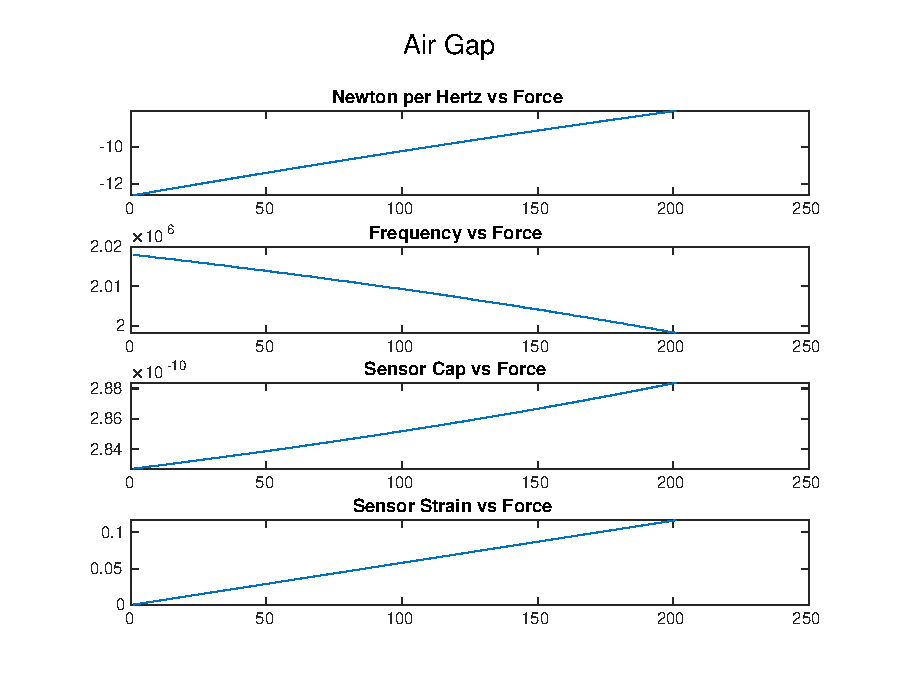
\includegraphics[width=0.6\textwidth]{appc_air_gap_plot.eps}
\caption{
Result of computation of device frequency and sensitivity over the required input range.
}
\label{fig:appc_airgap_graph}
\end{figure}

\begin{equation}\label{eq:air_gap_sense_c}
 \frac{df}{dF} = 
-\frac{0.0796\,A\,L\,e_{1}\,{e_{2}}^2}{\mathrm{ks}\,{\left(2.5000e-05\,e_{1}+e_{2}\,\left(\mathrm{d1n}-\frac{F}{\mathrm{ks}}\right)\right)}^2\,{\left(L\,\left(\mathrm{cb}+\frac{A\,e_{2}}{\mathrm{d2n}}+\frac{A\,e_{1}\,e_{2}}{2.5000e-05\,e_{1}+e_{2}\,\left(\mathrm{d1n}-\frac{F}{\mathrm{ks}}\right)}\right)\right)}^{1.5000}}
\end{equation}    

\pagebreak



%% Closed Area
A model was also used to explore the closed area sensor configuration. 
The resulting performance graphs are shown in \ref{fig:appc_closed_graph}.
The sensitivity is much greater for this model, requiring less Newtons to 
alter the resonant frequency in Hertz when compared to the air gap model.
For these calculations, the sensitivity can approach infinity as the region size
approaches zero. In reality, the device will continue to get stiffer as it compresses 
considerably, limiting the compression. The equation for the sensitivity to input force
is shown in \ref{eq:appc_d1}. The true sensor does not have completly linear characteristics,
but the sensitivity increases with greater force. Also, the sensitivity is approximately linear
with input force, so the response is roughly proportional to the square of the input force
for this configuration.
This model does not entirely capture the performance of the sensor during the rock cutting experiment,
but agrees with the trend that a more compressed sensor is more sensitive, 
and it shows sensitivity of similar magnitude.
The script and output are given in \ref{lst:closed1} and \ref{lst:closed2}, respectively.


\begin{figure}[ht]
\centering
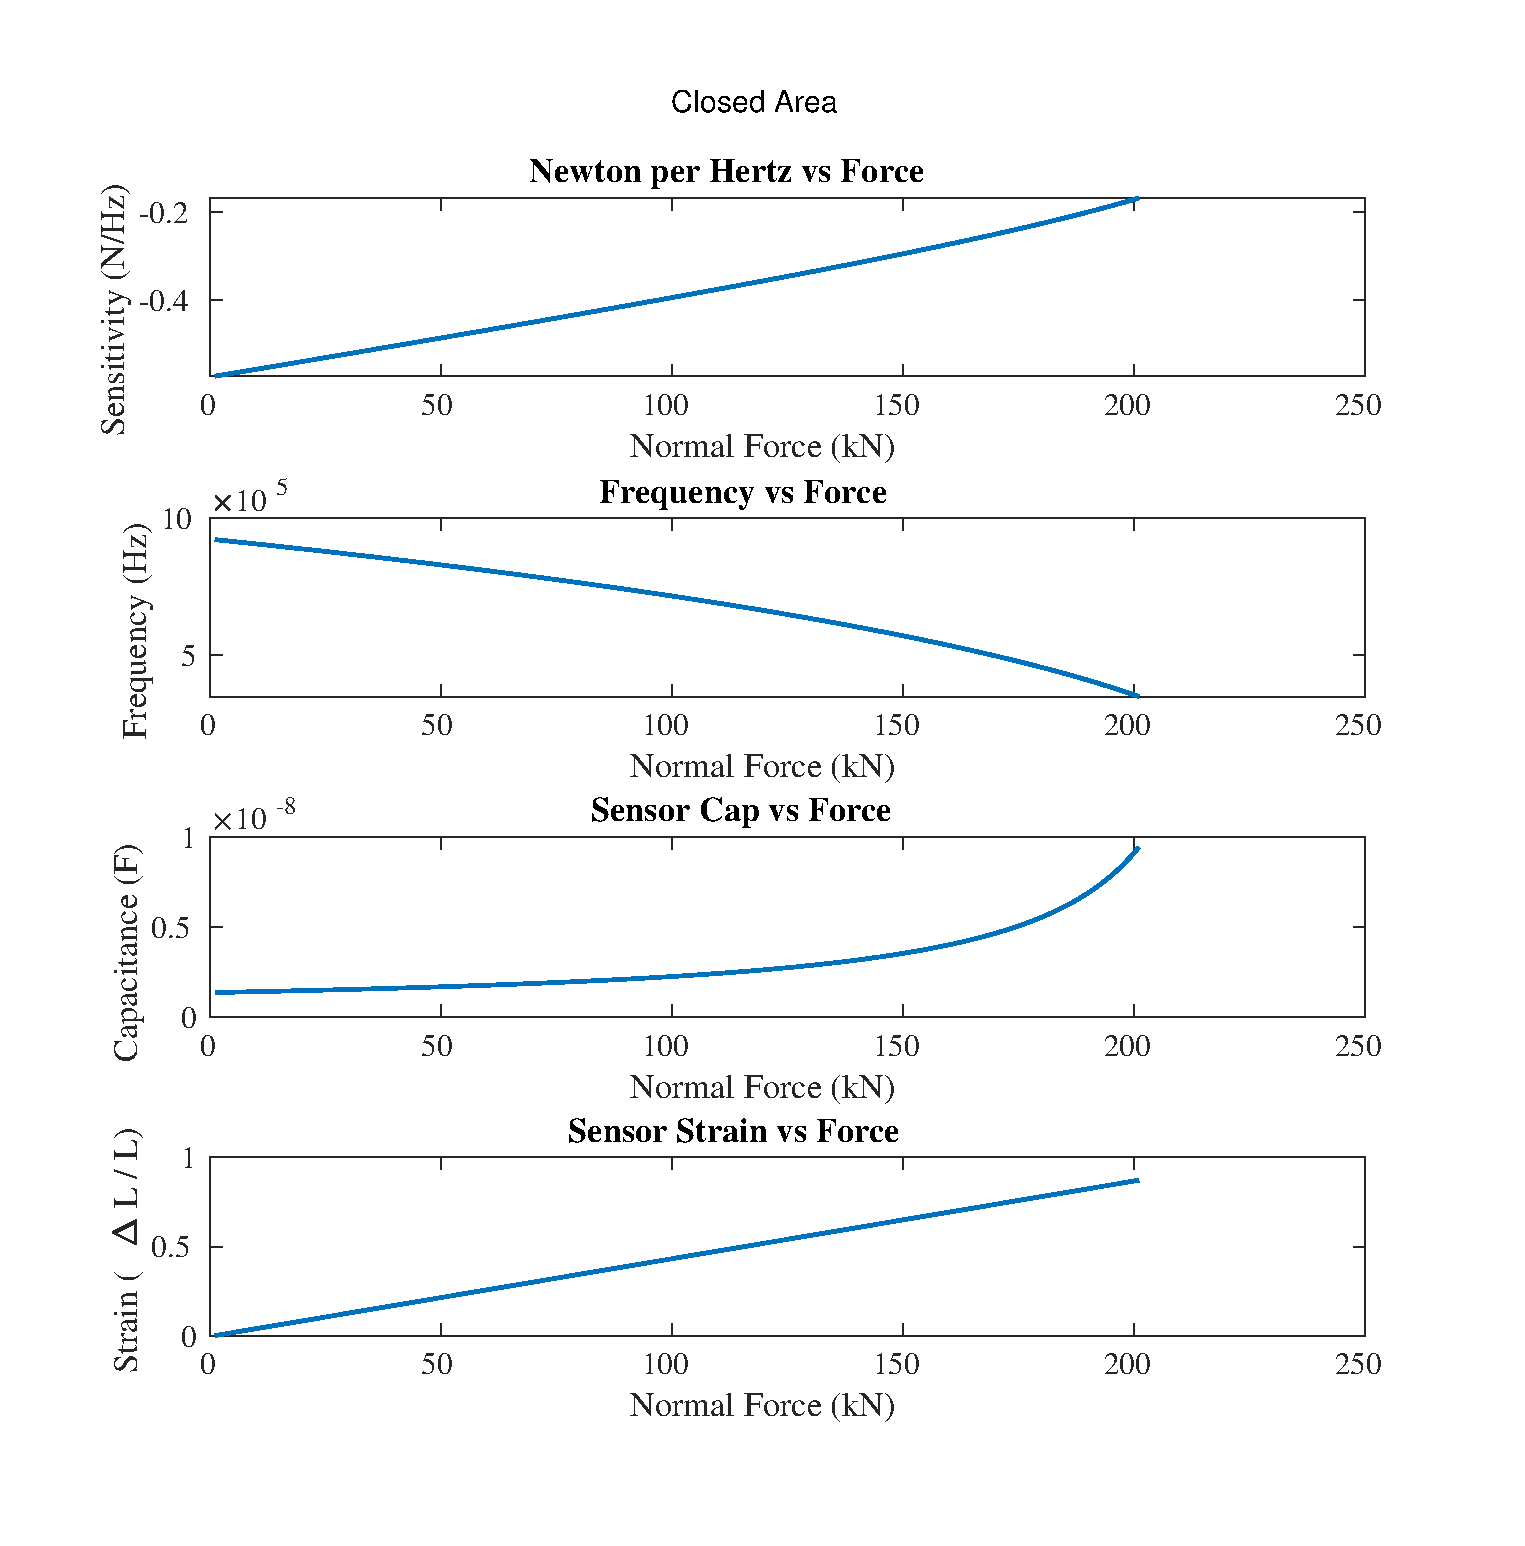
\includegraphics[width=0.6\textwidth]{appc_closed_gap_plot.eps}
\caption{
Result of computation of device frequency and sensitivity over the required input range.
}
\label{fig:appc_closed_graph}
\end{figure}

\begin{equation} \label{eq:appc_d1}
\frac{df_{r1}}{dF} = -\frac{0.0796\,L\,\left(\frac{A\,e}{k_{1}\,{\left(\mathrm{d1n}-\frac{F}{k_{1}}\right)}^2}+\frac{A\,e}{k_{2}\,{\left(\mathrm{d2n}-\frac{F}{k_{2}}\right)}^2}\right)}{{\left(L\,\left(\mathrm{cb}+\frac{A\,e}{\mathrm{d1n}-\frac{F}{k_{1}}}+\frac{A\,e}{\mathrm{d2n}-\frac{F}{k_{2}}}\right)\right)}^{1.5000}}
\end{equation}

\pagebreak

%% listings

\lstinputlisting[language=Matlab,label={lst:airgap1},caption={Script for modelling air gap}]{supporting-files/matlabs/airgap_script.m}

\pagebreak

\lstinputlisting[language=Matlab,label={lst:airgap2},caption={Output from air gap script}]{supporting-files/matlabs/airgap_output.txt}

\pagebreak

\lstinputlisting[language=Matlab,label={lst:closed1},caption={Script for modelling closed area}]{supporting-files/matlabs/closed_script.m}

\pagebreak

\lstinputlisting[language=Matlab,label={lst:closed2},caption={Output from closed area script}]{supporting-files/matlabs/closed_output.txt}



\end{document}